\subsection{Skyroads}
Bei dem Spiel \textit{Skyroads} von \textit{Bluemoon} ist eine Art Jump and Run Spiel aus dem Jahr 1993. Ziel des Spiels ist es ein Raumschiff durch einen Parcour zu manövrieren. Der Spieler muss hierbei über Hindernisse oder Abgründe springen, beziehungsweise diesen ausweichen. Schafft er das Level nicht, kann er es beliebig oft neu starten. Das Prinzip des Spiels stammt aus dem Spiel \textit{Kosmonauts}, welches von den gleichen Entwicklern bereits im Jahre 1989 veröffentlicht wurde. Zu Beginn des Spiels stehen dem Nutzer bereits alle Levels zur Verfügung. Er kann in einer Übersichtsseite das gewünschte Level auswählen. \\
Mit \textit{Skyroads XMAS-Special} wurde 1994 ein Nachfolger veröffentlicht. Außerdem existieren mittlerweile sehr viele andere Spiele, die nach einer ähnlichen Spielmechanik funktionieren.
\begin{figure}[ht]
	\centering
	\begin{subfigure}{6 cm}
	\centering
			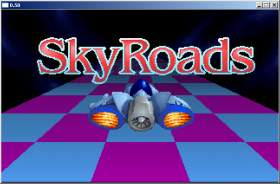
\includegraphics{gfx/recherche/skyroads1.jpg}
	\end{subfigure}
	\begin{subfigure}{6 cm}
	\centering
			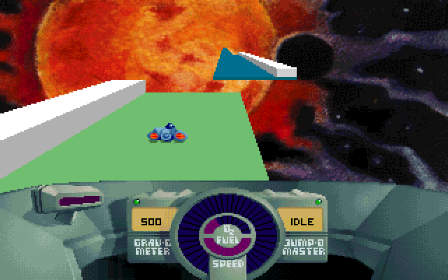
\includegraphics{gfx/recherche/skyroads2.jpg}  
	\end{subfigure}
	\caption{Skyroads}
\end{figure}\\

\subsection{AudioSmurveadelicForShizzleMyNizzle}
